%% 内容梗概

%% プリアンブル %%%%%%%%%%%%%%%%%%%%%%%%%%%%%%%%%%%%%%%%%%%%%%%%%%%%%%%%
\documentclass[a4j]{jarticle}

\usepackage{kut-abstract}
%\usepackage[dvips]{graphicx}
\usepackage[dvipdfmx]{graphicx}

%% 表題 %%%%%%%%%%%%%%%%%%%%%%%%%%%%%%%%%%%%%%%%%%%%%%%%%%%%%%%%%%%%%%%%
%% 注意! 情報学群生の場合は,以下の \ScInfo を有効にすること.
%\ScInfo        %% 情報学群生の場合

\Bachelor	%% 卒業研究論文梗概の場合
%\Project	%% プロジェクト研究報告書梗概の場合
%\Seminar	%% 特別研究セミナー課題研究報告書梗概の場合
%\Master	%% 修士学位論文(情報システム工学コース)梗概の場合
%\Doctorate	%% 博士学位論文(情報システム工学コース)梗概の場合
%\English	%% 英語の場合

\Eyears{2017}
\Etitle{English Title}
%\idnumber{}
\Eauthor{YAMASAKI, Naoyuki}
\Eaffiliate{Iwata Lab.}

%% 本文 %%%%%%%%%%%%%%%%%%%%%%%%%%%%%%%%%%%%%%%%%%%%%%%%%%%%%%%%%%%%%%%%

\years{平成29}
\title{LSTM-RNN用アクセラレータ回路の相互結合網の検討}
\idnumber{1180386}
\author{山 崎 ~~尚 之}
\affiliate{岩田研究室}

%% 本文 %%%%%%%%%%%%%%%%%%%%%%%%%%%%%%%%%%%%%%%%%%%%%%%%%%%%%%%%%%%%%%%%
\begin{document}
\begin{Abstract}

 \section{はじめに}

言語処理,音声認識の分野で長期短期記憶LSTM(Long Short-term Memory)が注目されており,
組込みシステムでリアルタイム翻訳などに用いる場合アクセラレータ回路を使用し,
高速に処理する必要がある.
%LSTMを用いた再起型ニューラルネットワーク
LSTM-RNN(Recurrent Neural Network)は
一般的な人工ニューラルネットワークANN(Artificial Neural Network)に比べ,
3種のゲートと自状態の重みが必要で演算量が大きくなる.
そのため,LSTM-RNN用アクセラレータの要求が求められるようになっている.

先行研究として,LSTMを含む微分可能ニューラルコンピュータDNC(Differentiable Neural Computer)
用単一コアの提案がされている\cite{bib:pre-method}.
しかし,シングルコアでは処理性能に限界があるためマルチコア化が求められる.

本研究では,LSTMをマルチコアで動作させる場合に必要な相互結合網回路での負荷の割り当て法について,
負荷を見積もり検討を行う.
また,見積もった性能が達成できているかFPGA上に実装し,
性能を評価する.



 \section{負荷割り当て方法の検討}
 負荷割り当ての方法を考える上で重要なLSTMの計算フローと並列処理の軸を図1に示す.
 \begin{figure}[h]
  \centering
  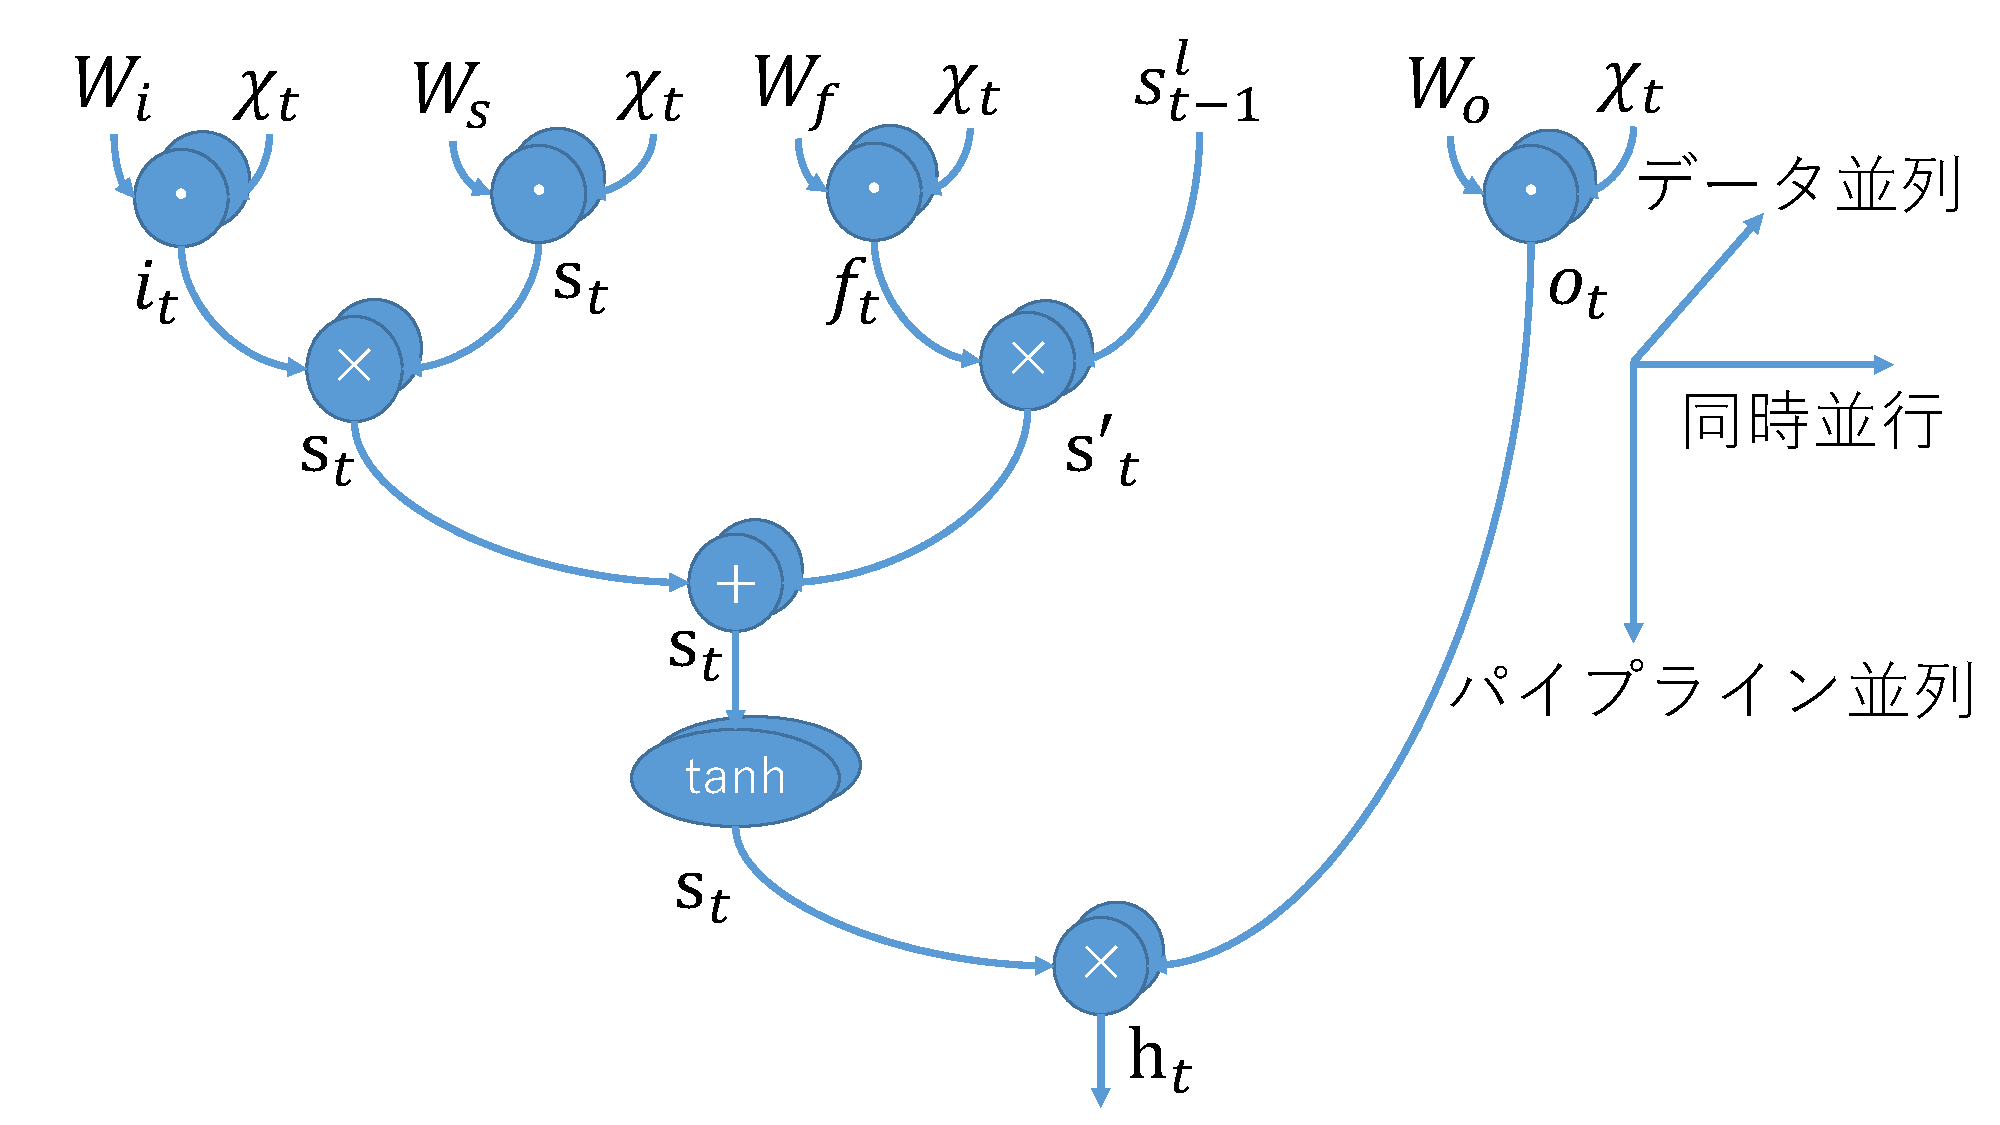
\includegraphics[width=5cm]{flow.jpg}
  \caption{LSTMの計算フロー図}
 \end{figure}


 並列処理の方法は以下の3方向にそった負荷割り当てが考えられる.

 \begin{itemize}
  \item 同時実行並列方向の負荷割り当て
  \item パイプライン並列方向の負荷割り当て
  \item データ並列方向の負荷割り当て
 \end{itemize}



この3つの負荷割り当て方法をコア数50,中間層のニューロン数200,入力数を50とし,
同時実行可能な時間の割合p,1対多の通信が可能な割合q,各コアに分割保存可能なデータの割合rを,
負荷の割り当てをしない場合とそれぞれ比較した結果を表1に示す.
\begin{table}[htb]
   \begin{center}
     \caption{各負荷割り当て方法の負荷見積もり}
     \begin{tabular}{|c||c|c|c|}\hline
      負荷割り当て方法 & p & q &  r \\ \hline
      同時実行並列 & 99.3\% &  5\% &  5\% \\ \hline
      パイプライン並列 & 99.3\% &  4\% &  4\% \\ \hline
      データ並列 & 99.9\% &  8\% &  8\% \\ \hline
    \end{tabular}
  \end{center}
\end{table}


表1より,すべての項目でデータ並列が高い負荷割り当てを実現していることが分かる.
ここで,q,rが低い値となっているのは,
分割数の変化に関係しないデータの割合が多くなるためと考えられる.

%応じて通信データの量は減少するが,
%割り当てられるデータの個数が増えるため負荷は一定
%通信データ量は少なくなるが,
%通信回数が多くなるためである.
次に、1番性能の高かったデータ並列方向の負荷割り当てに対し,ニューロン数と入力数,
コア数を変化させた場合の各コアのローカルメモリの削減割合を算出した結果を図2に示す.

\begin{figure}[h]
 \centering
 \includegraphics[width=5cm]{c50.jpg}
 \caption{コア50個の時のメモリ削減割合}
\end{figure}

図2よりLSTMのネットワーク規模が大きくなるにつれて,
メモリの削減割合が減少していることが分かる.
これは負荷割り当てが分割数に関係しないデータが他のデータに比べて,
中間層のニューロン数の総数に大きく影響されるためと考えられる.
%ネットワーク規模の二乗に比例して増加するためと考えられる.

 \section{まとめ}
負荷の割り当て方法として,
データ並列方向の負荷割り当てが3つの割り当て方法の中では最も高い性能が得られることが分かった.
しかし,ネットワーク規模が大きくなると負荷の削減割合が減少し性能が落ちることが分かった.
今回算出した結果は入出力にかかる処理時間などを考慮していない時の結果である.
よって今後より精密な見積もりを行い最適な負荷割り当て法を提案し,
それに適した相互結合網回路を設計し実装を行う.


%% 参考文献 %%%%%%%%%%%%%%%%%%%%%%%%%%%%%%%%%%%%%%%%%%%%%%%%%%%%%%%%%%%%
\begin{thebibliography}{99}
 \bibitem{bib:pre-method} Akane Saito, Yuki Umezaki, and Makoto Iwata, ``Hardware Accelerator for Differentiable Neural Computer and Its FPGA Implementation,'' Proceedings of the 2017 International Conference on Parallel and Distributed Processing Techniques and Applications(PDPTA'17), pp.232-238, July 2017.
\end{thebibliography}

\end{Abstract}
\end{document}
